\documentclass{ecai2010}
\usepackage{times}
\usepackage{graphicx}
\usepackage{latexsym, epstopdf, setspace, units, pgfplots}
\usepackage[algo2e, noend, noline, linesnumbered]{algorithm2e}
\DontPrintSemicolon
\newcommand{\pushline}{\Indp}% Indent
\newcommand{\popline}{\Indm}
\newcommand{\sgn}{\mathop{\mathrm{sgn}}}
\newcommand{\tuple}[1]{\ensuremath{\left \langle #1 \right \rangle }}
\setlength{\belowcaptionskip}{-15pt}
\ecaisubmission   % inserts page numbers. Use only for submission of paper.
                  % Do NOT use for camera-ready version of paper.

\begin{document}

\title{Quality-based Rewards for \\ Monte-Carlo Tree Search Simulations}

\author{Tom Pepels \and Marc Lanctot \and Mark~H.~M. Winands \institute{Maastricht University, Department of Knowledge Engineering, Maastricht, The Netherlands, email: \{tom.pepels,marc.lanctot,m.winands\}@maastrichtuniversity.nl} }

\maketitle
\bibliographystyle{ecai2010}

\begin{abstract}
In this paper measures for assessing the a posteriori quality of Monte-Carlo simulations are introduced. We show that altering the rewards of simulated play-outs in Monte-Carlo Tree Search based on their assessed quality improves results in five different two-player games. To achieve these results we propose two novel enhancements, the \emph{Qualitative Bonus} and the \emph{Relative Bonus}. The former relies on an domain-dependent assessment of the game's terminal state, whereas and the latter relies on the total number of moves made during a simulation. The proposed enhancements lead to a considerable performance increase in all five domains discussed.
\end{abstract}

%-------------------------------------------------------------------
\section{Introduction}
\label{sec:intro}
Monte-Carlo Tree Search (MCTS) is a best-first search method, based on random sampling of a given domain \cite{kocsis2006bandit, coulom2007efficient}. MCTS depends on the results of numerous simulations and grows a search tree online. Each of these consist of two parts, 1) the selection step, where moves are selected and played according to the a selection policy, and 2) the play-out step, where moves are played according to a simulation strategy. At the end of each play-out a terminal state is reached and the result $r$, usually expressed numerically in some discrete range, e.g. $r \in \{-1, 0, 1\}$ representing a loss, draw or win, respectively, is backpropagated along the tree from the expanded leaf to the root node. All rewards are colleced at the nodes on the first ply, on which the final move to play is based. which is selected based on either the node with the highest number of visits, the highest average reward, or a combination of these two \cite{chaslot2008progressive}. In this paper two methods are proposed for determining the quality of a simulation based on the terminal state reached. The first method proposed assesses the quality of a simulation based on its length $m_{ST}$. In the second method, we propose a heuristic evaluation of the terminal state $q$ to determine the simulation's quality. Moreover, we show that adjusting $r$ in a specific way using  $m_{ST}$ and/or $q$ leads to increased performance in five different two-player games.

Other techniques for rewarding simulations have been proposed \cite{Winands2010a}, where play-outs are cut-off early and their state heuristically evaluated. Furthermore, evaluating the final \emph{score} of a game has shown to improve results in games that base the winning player on the one with the highest score \cite{shibahara2008combining}. However, for some domains a strong heuristic evaluation may not be available or too time-consuming, and certainly not all games determine the winning player on the highest scoring player. Nonetheless, using the straightforward discrete reward $r$, any information other than the win/loss/draw state of the play-out's final position is disregarded. For these reasons, we propose assessing the rewards of play-outs based on any information available at the terminal state.

The paper is structured as follows; first, the general MCTS framework is discussed. Next, two different methods for assessing the quality of play-outs are detailed. In Section \ref{sec:qoreward} explains how rewards can be altered given using the quality measures from the previous section. Followed by pseudo-code outlining the proposed algorithm. Finally the performance of the proposed methods is determined in the experiments section, accompanied by a discussion and conclusion.

%-------------------------------------------------------------------
\section{Monte-Carlo Tree Search}
\label{sec:mcts}
\begin{figure}[ht]
	\centering
	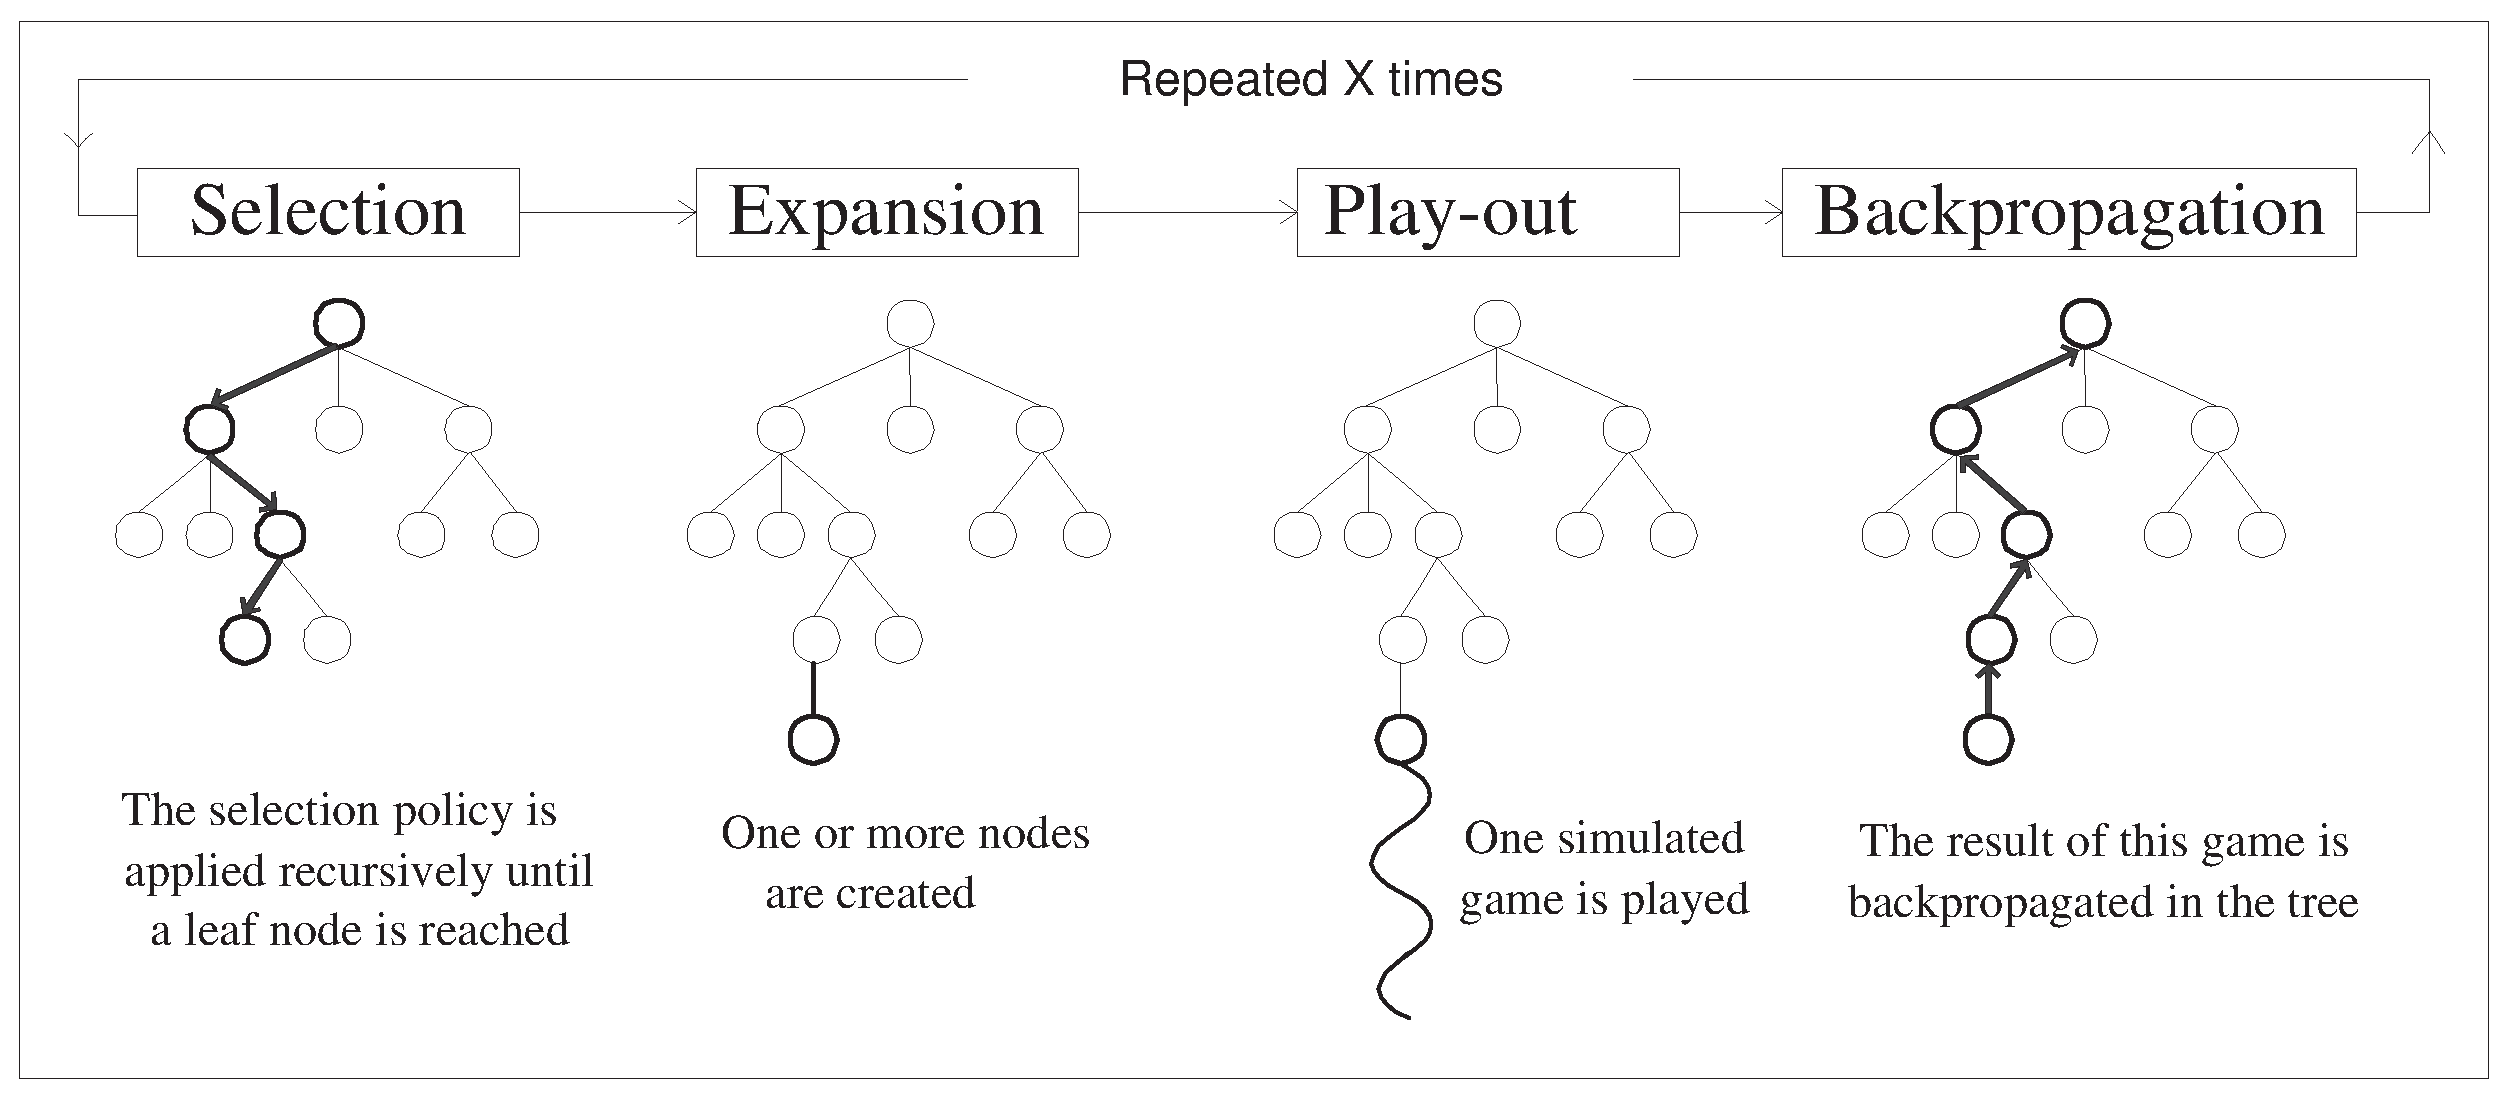
\includegraphics[width=.45\textwidth]{img/figure1.eps}
	\caption{Strategic steps of Monte-Carlo Tree Search \cite{chaslot2008progressive}.}
	\label{fig:mcts-algorithm}
\end{figure}
%from pac-man paper
Monte-Carlo Tree Search (MCTS) is a best-first search method based on random sampling of the state space for a specified domain \cite{kocsis2006bandit},\cite{coulom2007efficient}. In gameplay, this means that decisions are made based on the results of random play-outs. MCTS has been successfully applied to various two-player games games such as Go \cite{lee2010current} and Hex \cite{arneson2010monte}. Moreover, MCTS has recently seen successes in other domains such as Real-Time Strategy games \cite{browne2012survey}, Real-Time games such as Ms Pac-Man \cite{enhancementspacmancig12} and the Physical Travelling Salesman problem \cite{powleytsp}, and non-game domains such as optimization, scheduling and security \cite{browne2012survey}.

In MCTS, a tree is built incrementally over time and maintains statistics at each node corresponding the rewards collected at those nodes and number of times the nodes have been visited. The root of this tree corresponds to the agent's current position. The basic version of MCTS consists of four steps, which are performed iteratively until a computational threshold is reached, i.e. a set number of iterations, an upper limit on memory usage, or a time constraint. The four steps (depicted in Figure \ref{fig:mcts-algorithm}) at each iteration are \cite{chaslot2008progressive}:
\begin{itemize}
\item {\bf Selection}. Starting at the root node, children are chosen according to a selection policy (described in Subsection \ref{subsec:uct}). When a leaf node is reached that does not represent a terminal state it is selected for expansion.
\item {\bf Expansion}. All children are added to the selected leaf node given available moves.
\item {\bf Play-out}. A simulated play-out is run, starting from the state of the added node. Moves are performed randomly or according to a heuristic strategy until a terminal state is reached.
\item {\bf Backpropagation}. The result of the simulated play-out is propagated immediately from the selected node back up to the root node. Statistics are updated along the tree for each node selected during the selection step and visit counts are increased.
\end{itemize}
The combination of moves selected during the selection and play-out steps form a single simulation. In its basic form, MCTS requires no heuristic state evaluation. Nonetheless, in most cases it is beneficial to add some domain knowledge for selecting moves to play during play-out. MCTS can be terminated anytime and select a move to play based on the rewards and visits collected on the first ply.
% /from pac-man paper

%-------------------------------------------------------------------
\subsection{UCT}
\label{subsec:uct}
%from pac-man paper
During the selection step, a policy is required to explore the tree for rewarding decisions and finally converge to the most rewarding one. The Upper Confidence Bound applied to Trees (UCT) \cite{kocsis2006bandit} is derived from the UCB1 policy \cite{auer2002using} for maximizing the rewards of a multi-armed bandit. UCT balances the exploitation of rewarding nodes whilst allowing exploration of lesser visited nodes. Consider a node $p$ with children $A(p)$, then the policy determining which child $i$ to select:
\begin{equation}
\label{eq:uct}
i^* = argmax_{i \in A(p)}\left\{ v_i + C \sqrt{ \frac{\ln{n_p}}{n_i}}\right\}
\end{equation}
where $v_i$ is the score of the child $i$ based on the average result of simulations that visited it. $n_p$ is the visit count of the node and $n_i$ the visit count of the current child. $C$ is the exploration constant to be determined by experimentation.
% /from pac-man paper

\section{Assessing simulation quality}
\label{sec:poqual}

In this section two measures by which the quality of the terminal state of a simulation can be assessed are discussed. First, the length of a simulation is detailed as a quality measure, second some heuristic assessment of terminal states is considered. In the next section we establish how these techniques can be used to enhance the rewards of MCTS simulations.

The first, straightforward assessment of a simulation's quality is the length of the game played. Consider a single MCTS simulation as depicted in Figure \ref{fig:mcts-simulation}, here we can define two seperate distances: 
\begin{enumerate}
\item The number of nodes between the root node $S$ to the expanded leaf $N$, $d_{SN}$,
\item The number of moves required to reach $T$, the terminal state, from $N$ during play-out $d_{NT}$.
\end{enumerate}
The length of the simulation is then defined as the sum of these distances:
\begin{equation}
m_{ST} = d_{SN} + d_{NT}
\label{eq:m_ST}
\end{equation}
i.e. the total number of moves made by both players before reaching the terminal state of the game $T$ from $S$, the root's game state.

\begin{figure}[t]
	\centering
	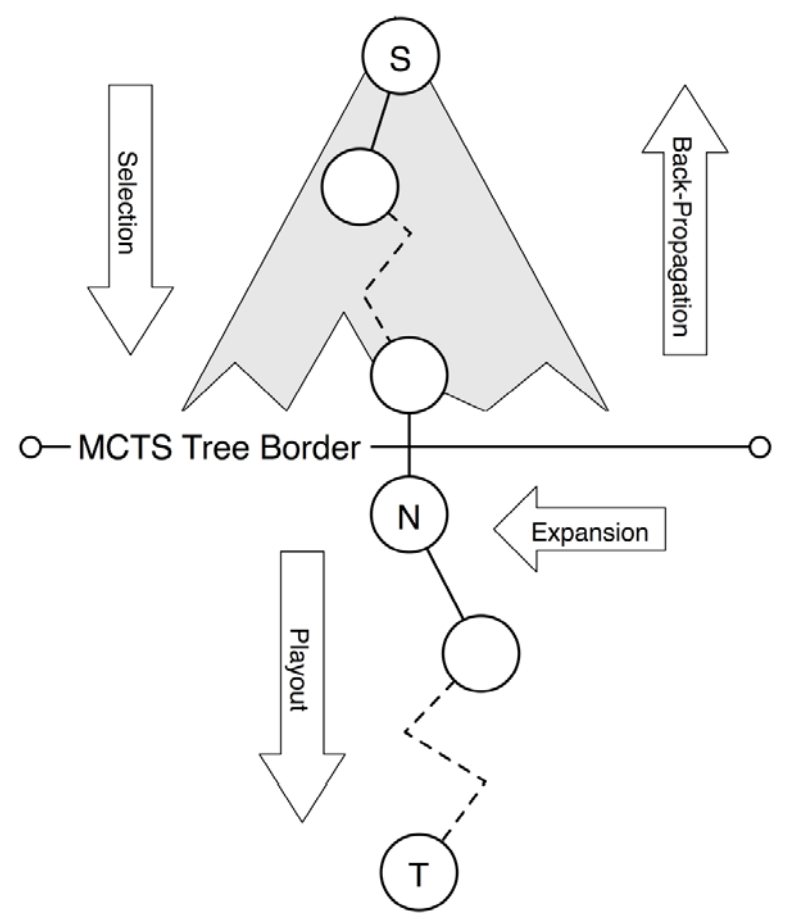
\includegraphics[width=.3\textwidth]{img/figure2.png}
	\caption{A single MCTS simulation \cite{finnsson2010learning}.}
	\label{fig:mcts-simulation}
\end{figure}

Moves selected during play-out are generated by some simulation strategy. Generally this aither a  random strategy, or a rule-based, reactive strategy, combined with a source of randomness such as an $\epsilon$-greedy selection \cite{sutton1998reinforcement, sturtevant2008analysis}. Various alternative methods have been proposed, such as using low-level $\alpha\beta$ searches \cite{winands2011a}, and methods that learn a strategy online, such as N-Grams and the Last-Good-Reply policy \cite{Tak2012}, or the Move-average Sampling Technique (MAST) \cite{finnsson2010learning}. However, each of these methods and strategies have some random element in common. Moreover, they select moves based on some imperfect technique, because they have to make quick decisions to allow for numerous simulations to be made during the allowed time. As such, each move played ultimately increases uncertainty with respect to the accuracy of the final result, by some degree. Hence, the length of the simulation may be regarded as an indicator of the accuracy of its result.

A predominant benefit of using simulation length as a quality measure is that it can be applied independent of the domain. Unless the game's length is fixed, the variance of the length of a play-out in particular can be informative in determining its quality.

The second measure of a simulation's quality is based on a heuristic assessment of the game's terminal state. Although evaluation functions can be designed for most games, they're used to evaluate non-terminal positions and assign them a specific value. However, MCTS generally performs a play-out until a terminal state is reached. Therefore, we are interested in assessing the terminal state of a game rather than intermediary positions. This limits the number of features that can be evaluated, yet provides a direct application to MCTS.

As before, consider a single MCTS simulation as depicted in Figure \ref{fig:mcts-simulation}. When the terminal state $T$ is reached, an quality assessment function is called to evaluate the position with respect to the winning player. This measure; $q \in (0, 1)$ should reflect the quality of the terminal state. For instance, in a game with material such as Breakthrough, Chess or Checkers, an evaluation can be based on scoring the remaining material of the winning player. For a such as Chinese Checkers, the inverse of the number of pieces the opponent has in his target base can be considered. As such, the quality is based on the a posteriori evaluation of the terminal state. Having witnessed the game progress from $S$ to $T$ the score is based on an evaluation of $T$ given the progression $S \ldots N \ldots T$.

%-------------------------------------------------------------------
\section{Quality-based simulation rewards}
\label{sec:qoreward}
Based on the classification of quality measures in the previous section, we propose two reward alterations for MCTS: the \emph{Relative Bonus} and the \emph{Qualitative Bonus}, relating to the length of the simulation and the heuristic evaluation of the terminal state, respectively. 

In our proposed framework, rewards of MCTS simulations return a tuple of three reward values, $\tuple{r, w, q, d_{NT},}$ representing the reward $r \in \{-1, 0, 1\}$, the winning player $w$, the heuristic assessment of the terminal state $q$, and the distance from the expanded node $N$ to the terminal state $T$: $d_{NT}$, respectively. $m_{ST}$ is then computed as defined in \ref{eq:m_ST}. First we will define the Relative Bonus (RB) based on $m_{ST}$ information, after which, the Qualitative Bonus (QB) is described which is similar, except for being based on $q$.

\subsection{Relative Bonus}
First, note that $m_{ST}$ depends considerably on both the domain in question and the progress of the game. By itself, the variable is neither normalized, nor relative to a central tendency. As such, adding the value to $r$ as is, leads to a biased distribution of the value over time, where, at the beginning of a game, $m_{ST}$ takes on higher values than when the game approaches its terminal state. Moreover, considering that the length of a game cannot be determined beforehand, we have no accurate way of normalizing the observed values absolutely, based on the expected total length of the game. Therefore, two normalizers need to be approximated: 1) a central measure, to relate the desired variable to the current progress, and 2) a normalizing distance to the central measure, since the variance of observed $m_{ST}$ values may also differ over time.

A central measure can be approximated online, by maintaining an average $\bar{M}$, for each player (indexed by $w$), of the observed $m_{ST}$ values so far. After each simulation ends, $m_{ST}$ is compared to $\bar{M}^w$, and $\bar{M}^w$ is updated with the observed $m_{ST}$.
\begin{equation}
\delta_m = \bar{M}^w - m_{ST}
\end{equation}
%\begin{equation}
%\bar{M}^w_n = \bar{M}^w_{n-1} + \frac{m_{ST, n} - \bar{M}^w_{n-1}}{n}
%\end{equation}
 This ensures $\delta_m$ is relative to the current progress of the game, and independent of the domain's tendency regarding the length of games. Moreover we achieve the desired effect of valuating simulations shorter than average with a positive value and those longer with a negative value. However, $\delta_m$ still depends on the progress of the game. In most domains, the start of any game will have a high variance with respect to the length of simulations. Insufficient prior moves have been made, and MCTS can not yet accurately predict the progression of the game. As a consequence, play-outs will last longer at the start of the game than when it reaches the terminal state. As such the variance of the observed $m_{ST}$ values over time may differ substantially. Which leads to the requirement of a normalizer.

Assuming that the distribution of $m_{ST}$ values over time is $M \sim \mathcal{N}(\bar{M}, \hat{\sigma}_m)$, then $\hat{\sigma}^w_m$ is the sample standard deviation which can be used to normalize $\delta_m$ with respect to the current variance of the length of simulated games. Now we can define a normalized variable $\lambda$ as follows:

\begin{equation}
\lambda = \frac{\delta_m}{\hat{\sigma}^w_m}
\end{equation}

$\lambda$ is both normalized with respect to the sample standard deviation of $M$, and relative to $\bar{M}^w$. This means $\lambda$ wil be both independent of the progress of the game, and normalized with respect to the current variance in the length of simulations.

Since the distribution of $M$ is not known, $\lambda$ can still take on unrestricted values, particularly if $M \sim \mathcal{N}(\bar{M}, \hat{\sigma}_m)$ is close to uniform. Moreover, the relation with the desired reward is not neccesarily linear. As such, in order to both bound, and shape the values of the relative bonus $b_r$ we propose to use a sigmoid function centered around $0$ on both axes, and with a range of $[-0.25, 0.25]$.

\begin{equation}
b(\lambda) = -0.25 + \frac{0.5}{1+e^{-k\lambda}}
\label{eq:sigmoid}
\end{equation}

Figure \ref{fig:sigmoids} shows the graphs for three different values of $k$ in Equation \ref{eq:sigmoid}. $k$ is a constant to be determined empirically, which shapes the bonus to be added to $r$. Higher values of $k$ determine both the slope, and the start of the horizontal asymptotes of the sigmoid function.

\begin{figure}[t]
\centering
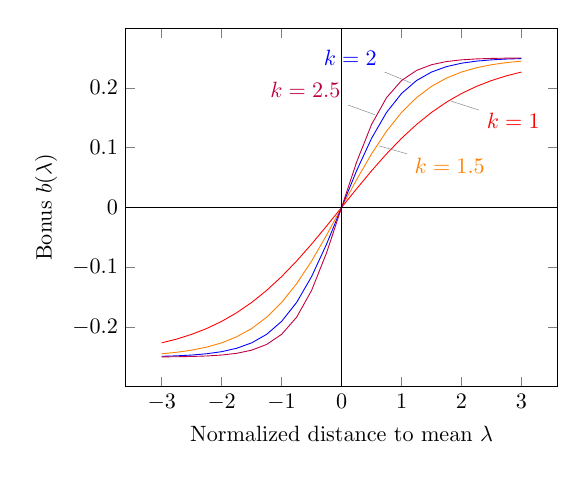
\begin{tikzpicture}[scale=0.8]
  \begin{axis}[
	ylabel = Bonus $b(\lambda)$,
    xlabel = Normalized distance to mean $\lambda$,
  	axis equal image=false 
  	]

    \addplot[red, mark=none, domain =-3:3] {.5/(1+e^(-x)) - .25} node [pos=0.8,pin={-10:$k=1$},inner sep=0pt]{};
    \addplot[orange, mark=none, domain =-3:3] {.5/(1+e^(-1.5*x)) - .25} node [pos=0.6,pin={-10:$k=1.5$},inner sep=0pt]{};
    \addplot[blue, mark=none, domain =-3:3] {.5/(1+e^(-2*x)) - .25} node [pos=0.7,pin={-200:$k=2$},inner sep=0pt]{};
       \addplot[purple, mark=none, domain =-3:3] {.5/(1+e^(-2.5*x)) - .25} node [pos=0.6,pin={-200:$k=2.5$},inner sep=0pt]{};
    \draw[ultra thin] (axis cs:\pgfkeysvalueof{/pgfplots/xmin},0) -- (axis cs:\pgfkeysvalueof{/pgfplots/xmax},0);
	\draw[ultra thin] (axis cs:0,\pgfkeysvalueof{/pgfplots/ymin}) -- (axis cs:0,\pgfkeysvalueof{/pgfplots/ymax}); 
  \end{axis}
\end{tikzpicture}
    \caption{Bonusses resulting from different $k$ constants in Equation \ref{eq:sigmoid}.}
	\label{fig:sigmoids}
\end{figure}

Finally, the reward $r$ returned by the original simulation is altered by $b(\lambda)$ as follows:
\begin{equation}
r_b = r + \sgn(r) \times b(\lambda)
\end{equation}

This value is backpropagated from the expanded leaf to the root node. The range of $r_b$ is now $[-1.25, 1.25]$, i.e. the bonus $b(\lambda)$ is centered around the possible values of $r$.

\subsection{Qualitative Bonus}
Calculation of the Qualitative Bonus follows the same procedure as the Relative Bonus. Similar to RB, a distribution over observed $q$ values is maintained $Q \sim \mathcal{N}(\bar{Q}, \hat{\sigma}_q)$ for each player $w$. The value of $q$ is determined by a domain dependent assessment of quality of the terminal state. Assuming that higher values of $q$ represent a higher quality terminal state for the winning player $w$, then $\delta_q$ becomes:
\begin{equation}
\delta_q = q - \bar{Q}^w
\end{equation}
Where $\bar{Q}^w$ is updated with $q$ after every simulation. Consequently, $\lambda$ is redefined as:
\begin{equation}
\lambda = \frac{\delta_q}{\hat{\sigma}^w_q}
\end{equation}
Finally the bonus $b(\lambda)$ is computed using the sigmoid function in equation \ref{eq:sigmoid} with an optimized $k$ constant, and summed with the result of the simulation $r$.

%-------------------------------------------------------------------
\section{Pseudo-Code}

Explain all the alterations to standard MCTS

\begin{algorithm2e}[ht]
\setstretch{1.15}
  {\bf MCTS}(node $p$, cumulative node depth $d_{Sp}$):\;
  \pushline
    \If{isLeaf($p$)}{Expand($p$)}
    Select a child $i$ according to Eq.~\ref{eq:uct} 	\;
    $d_{Si} \gets d_{Sp} + 1$								\;
    \eIf{$n_i = 0$}{
    	$\tuple{r, w, q, d_{iT}} \gets$ Playout$(n_i)$ 					\;			\label{alg:results}
    	$m_{ST} \gets d_{Si} + d_{iT}$									\;
    	\If{enabled$(b_r)$}{
    		$r \gets r + \sgn(r) \times$ BONUS$(\bar{M}^w - m_{ST}, \hat{\sigma}^w_m)$ 		\;
    		Update $\bar{M}^w$ and $\hat{\sigma}^w_m$ with $m_{ST}$						\;
		}
		\If{enabled$(b_q)$} {
    		$r \gets r + \sgn(r) \times$ BONUS$(q -\bar{Q^w}, \hat{\sigma}^w_q)$ 		\;
    		Update $\bar{Q^w}$ and $\hat{\sigma}^w_q$ with $q$ 						\;
    	}
    	Update node $i$ with $r$
    }{
    	$r$ = -MCTS($i$, $d_{Si})$)								\; 
    }
    Update node $p$ with $r$													\;
   \popline
    {\bf return} $r$													\;
  	\;
    {\bf BONUS}(distance to mean $\delta$, sample std. dev. $\hat{\sigma}$):			\;
    \pushline
    	$\lambda \gets \nicefrac{\delta}{\hat{\sigma}}$								\;
    	$b \gets \nicefrac{0.5}{\left(1+\exp(-K\lambda)\right)} - 0.25$					\;
    \popline
    \bf{return} $b$														\;
  \vspace{0.3cm}
  \caption{Pseudo-code of the MCTS and BONUS functions \label{alg}}
\end{algorithm2e}

%-------------------------------------------------------------------
\section{Experiments}
Experiments run on 5 different two-player games.
\subsection{Experimental setup}
Describe setup of experiments, k's used, c's used.

\subsection{Results}
- Results UCT vs RB
- Results UCT vs QB
- Results UCT vs RB + RB
- Results RB vs QB
- Graph of K's / UCT C's

%-------------------------------------------------------------------
\section{Conclusion}
Relative bonus - interesting because requires no domain knowledge, works best in games with long play-outs.
QB works in all domains, but requires domain knowledge, nonetheless, even using simple evaluation of the terminal state improved results considerably.

RB especially interesting for General Game Playing (GGP), where knowledge of games is sparse. RB improves results without domain-dependent knowledge.

Would be interesting to determine if RB/QB could improve results in non-game domains.

%-------------------------------------------------------------------
\subsection*{Acknowledgments}
This work is partially funded by Scientific Research (NWO) in the framework of the project Go4Nature, grant number 612.000.938.
\bibliography{references}
\end{document}